\chapter{Hardware}
In wat volgt, worden alle componenten uitvoerig besproken en wordt een verantwoording gegeven van de ontwerpskeuzes.

\section{Ultra Wide Band}  \label{sec:uwb}
In theorie is het mogelijk om de drone op een gekende locatie te laten vertrekken en een voorgeprogrammeerde route mee te geven. In de praktijk zorgt dat zeker en vast voor problemen. Denk bijvoorbeeld maar aan een ongekend obstakel dat plots het pad van de drone kruist, of een ventilatieschacht die hem uit positie blaast. Daarom is het nodig dat z'n precieze lokatie in de ruimte op elk moment gekend is. Veelgebruikte localisatietools zoals gps, wifi en bluetooth zijn te onnauwkeurig voor deze toepassing. Als de drone tussen 2 rekken met een doorgang van \SI{1}{\m} moet kunnen vliegen, dan moet de localisatie veel naukeuriger gebeuren.\\

Ultra Wide Band komt deze noden tegemoet. Dit is een vrij recente techniek met een nauwkeurigheid in de grootteorde van \SI{0.10}{\m}, wat volstaat om de drone indoor te kunnen lokaliseren.\\

Om deze lokatiebepaling via UWB te kunnen doen zijn 2 verschillende hardwarecomponenten noodzakelijk, namelijk enkele anker nodes (die op gekende locaties in het magazijn worden opgehangen) en een mobiele tag (die als onderdeel van de controller op de drone wordt bevestigd). Over de mobiele tag is meer te vinden in sectie \ref{sec:decawave}.

\section{Controller} \label{sec:controller}
\subsection{DecaWave DWM1001}  \label{sec:decawave}
De mobiele tag kan dan om de beurt de verschillende ankers aanspreken, en vragen hoe ver hij van hen verwijderd is. Wanneer er enkele afstanden gekend zijn, kan hij zijn locatie bepalen ten opzichte van de ankers.\\

De DecaWave DWM1001 bevat dezelfde UWB chip als de Pozyx tag, maar is goedkoper, compacter, en lichter. Voor de gebruikte drone is het minieme gewichtsverschil niet echt een probleem. Men moet echter wel in het achterhoofd houden dat meer massa de stabiliteit en vliegminuten in negatieve zin be\"invloedt.\\

RX Peak Current: \SI{154}{\mA} RX Mean Current: \SI{134}{\mA} TX Peak Current \SI{111}{\mA} TX Mean Current \SI{82}{mA}, \SI{2.8}{\V}-\SI{3.6}{\V}, \SI{0.55}{\W}\\
\SI{3}{\g}

\subsection{Raspberry Pi Zero W} \label{sec:raspberry_pi}
\SI{150}{\mA}, \SI{5.0}{\V}, \SI{0.75}{\W}\\
\SI{9}{\g}

\subsection{Lithium-ion Polymeer Batterij en Power Supply} \label{sec:lipo}
De Lithium-ion Polymeer Batterij (LiPo) moet de controller gedurende ongeveer een kwartier van stroom kunnen voorzien.\\
Een batterij met \SI{150}{\mA\hour} kan gedurende \SI{15}{\minute} zo'n \SI{600}{\mA} aan de controller leveren, de controller heeft ongeveer \SI{350}{\mA} nodig.\\
\SI{3.7}{\V}
\[\frac{\SI{1.30}{\W}}{\SI{3.7}{\V}}=\SI{350}{\mA}\]
\[\SI{350}{\mA}*\SI{0.25}{\hour}=\SI{87.5}{\mA\hour}\]\\
\SI{5}{\g}\\
\\
\textit{LiPo SHIM???}

\subsection{Totaal} \label{sec:totaal}
Totaal verbruik: \SI{1.30}{\W}\\
Totaal gewicht: \SI{25}{\g}

\section{Drone} \label{sec:drone}
Parrot AR.Drone 2.0 Elite Edition\\

De camera op de drone zou kunnen dienen om barcodes in te scannen, maar dat onderdeel werd niet onder de doelstellingen van dit project gedefini\"eerd.

\section{Setup} \label{sec:setup_hardware}
Op figuur \ref{fig:setup_hardware} vindt u de hardware setup.
\begin{figure}[p]
	\centering
	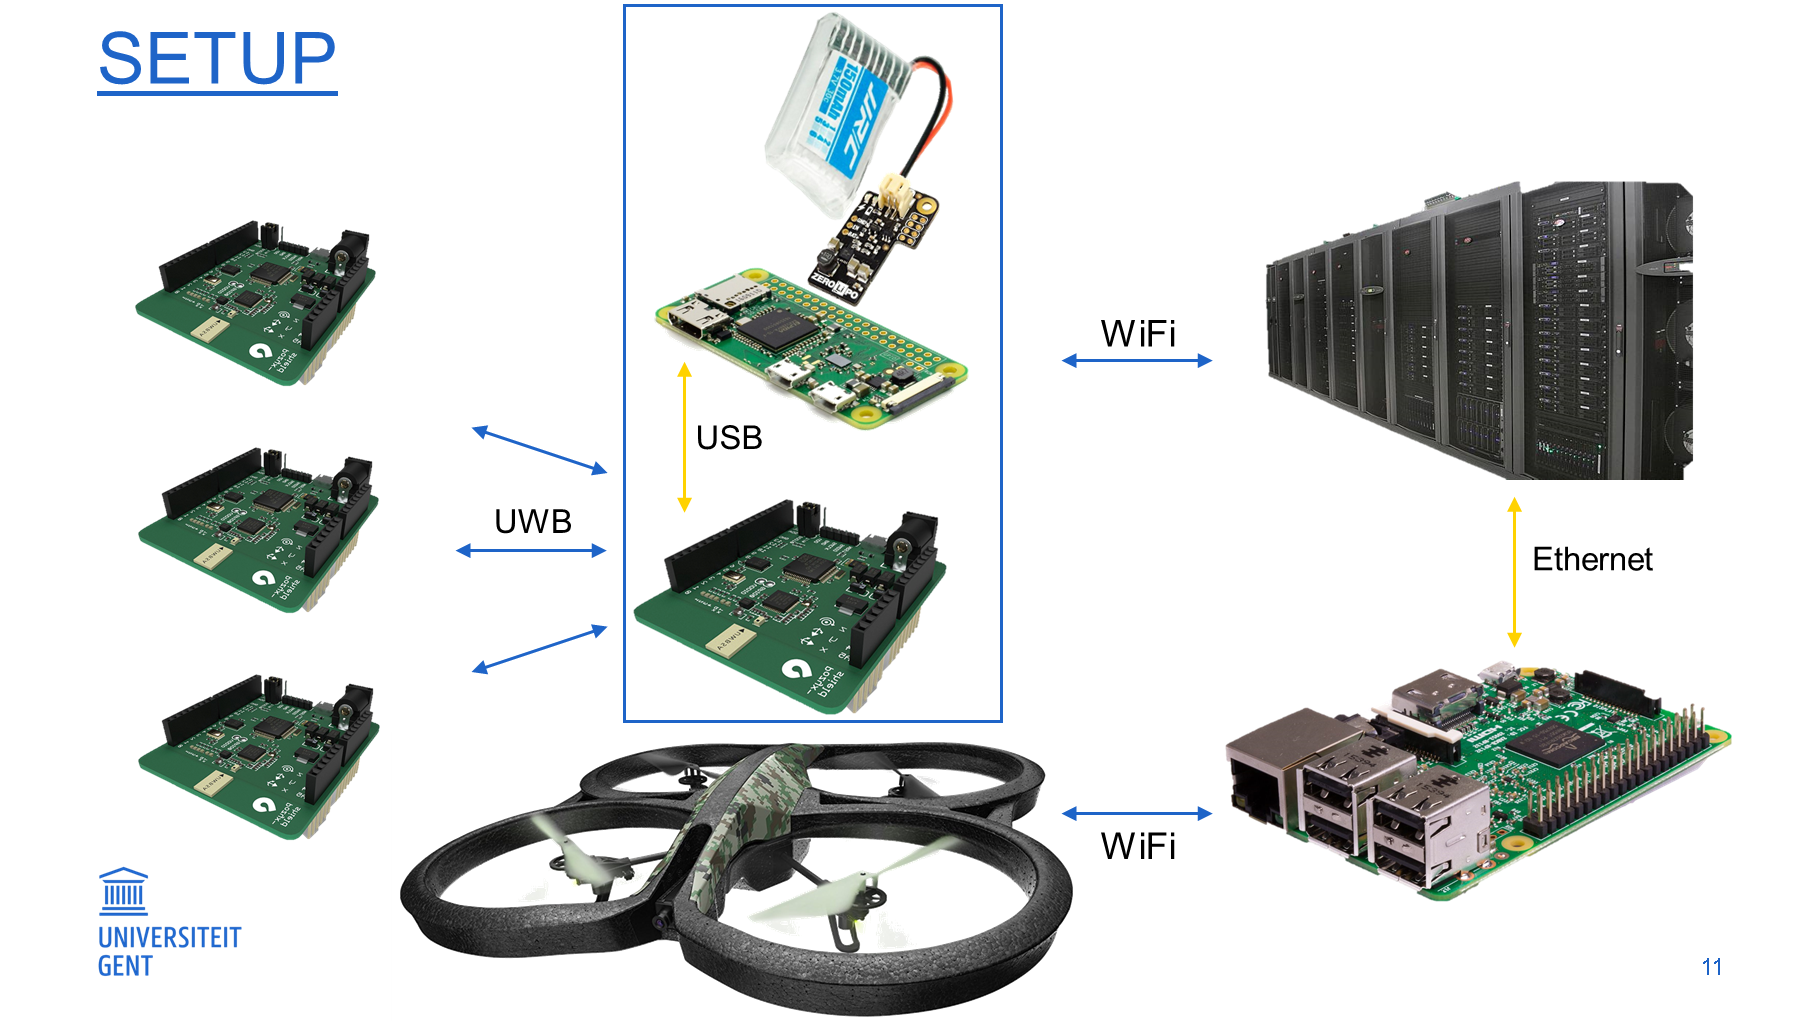
\includegraphics[width=\textwidth]{Setup_Hardware}
	\caption[Hardware setup]{Hardware setup.}
	\label{fig:setup_hardware}
\end{figure}
